\documentclass{beamer}

%For SQL highlighting
\usepackage{listings}
\usepackage{color}
\usepackage{animate}
\definecolor{dkgreen}{rgb}{0,0.6,0}
\definecolor{gray}{rgb}{0.5,0.5,0.5}
\definecolor{mauve}{rgb}{0.58,0,0.82}
\newcommand{\mycomment}[1]{}
\lstset{language=SQL,
  basicstyle={\small\ttfamily},
  belowskip=3mm,
  breakatwhitespace=true,
  breaklines=true,
  classoffset=0,
  columns=flexible,
  commentstyle=\color{dkgreen},
  framexleftmargin=0.25em,
  frameshape={}{yy}{}{}, %To remove to vertical lines on left, set `frameshape={}{}{}{}`
  keywordstyle=\color{blue},
  numbers=none, %If you want line numbers, set `numbers=left`
  numberstyle=\tiny\color{gray},
  showstringspaces=false,
  stringstyle=\color{mauve},
  tabsize=3,
  xleftmargin =1em
}

\title{Analysis of J-PAS}
\date{\today}

\begin{document}

\frame{\titlepage}

\mycomment{
\begin{frame}
\frametitle{Slide Title}
Steps:
\begin{itemize}
    \item Extracted JPAS objects from the J-PAS-mini database 
    \item Mathced with the SDSS objects (short description of the matching process)
    \item Selected the objects with spectum in the SDSS database
    \item Resampled the JPAS and the SDSS specta to the same wavelength grid. (short description of the resampling process)
    \item Compared the JPAS and the SDSS spectra (short description of the comparison results)
    \item Future work: (short description of the future work)
\end{itemize}

insert numbers of JPAS objects, SDSS objects, and the number of matched objects
objects with spectra in the SDSS database

\end{frame}
}

\begin{frame}
\frametitle{Project Overview}
\begin{itemize}
    \item Developed Python scripts to extract and process astronomical data.
    \item Utilized the J-PAS-mini database to gather JPAS objects.
    \item Implemented matching algorithms to correlate JPAS objects with SDSS objects.
    \item Performed data cleaning and preprocessing to ensure data quality.
    \item Conducted spectral analysis by resampling and comparing spectra from JPAS and SDSS.\@
    \item Generated visualizations to illustrate the comparison results.
    \item Documented the workflow and results for future reference and reproducibility.
\end{itemize}
\end{frame}

\begin{frame}
\frametitle{Extracting JPAS Objects}
    We extracted JPAS objects from the J-PAS-mini database, using SQL queries and Python scripts. We got 64293 objects.
    Used J-PAS-mini tables: 
    \begin{itemize}
        \item FLambdaDualObj (All astronomical objects that was detected in the J-PAS-mini survey and for which detection and aperture definition was performed using SExtractor)
        \item Filter (Table about the filters used in the J-PAS-mini survey)
    \end{itemize}
\end{frame}

\begin{frame}
    \frametitle{Extracting JPAS Objects}
    \begin{figure}[h]
        \centering
        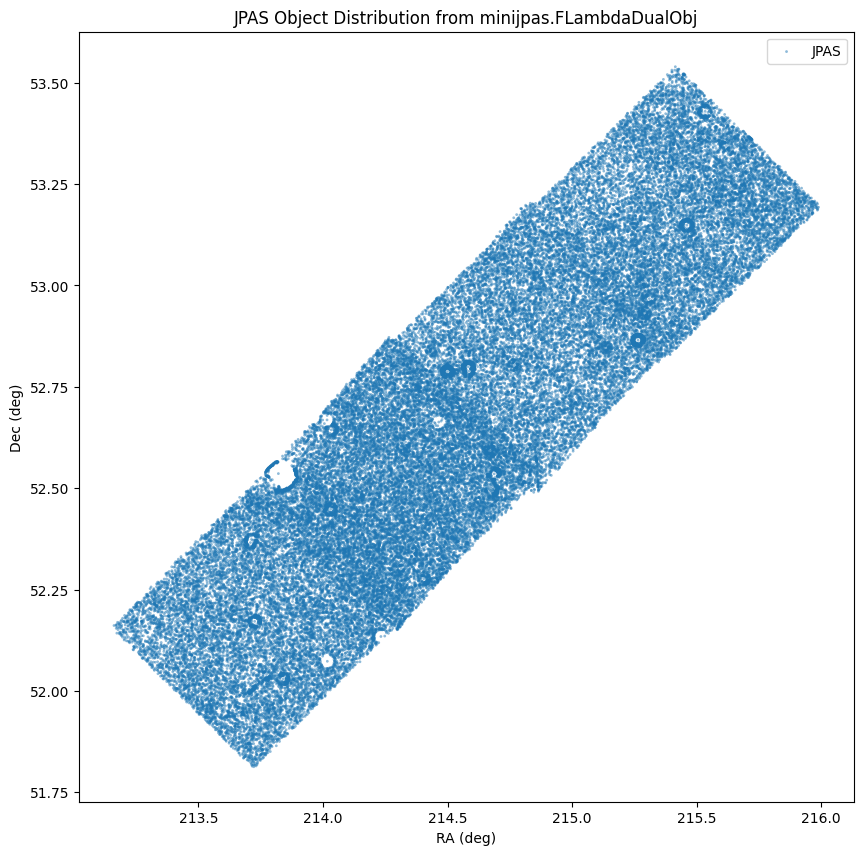
\includegraphics[width=0.8\textwidth]{../images/JPAS (FLambdaDualObj).png}
    \end{figure}
\end{frame}

\begin{frame}[fragile]
    \frametitle{Matching with SDSS Objects}
    To match JPAS objects with SDSS objects, first extracted SDSS objects from the SDSS database, using SQL query:
    \begin{lstlisting}
    SELECT 
    p.objid, p.ra, p.dec, p.u, p.g, p.r, p.i, p.z, p.run, p.camcol, p.field, p.specObjID 
    FROM PhotoPrimary AS p 
    WHERE p.ra BETWEEN {df_dual['ALPHA_J2000'].min()} AND {df_dual['ALPHA_J2000'].max()} 
    AND p.dec BETWEEN {df_dual['DELTA_J2000'].min()} AND {df_dual['DELTA_J2000'].max()} 
    AND p.r BETWEEN 14 AND 22.0
    \end{lstlisting}
    We got 35030 objects from the SDSS database.
\end{frame}

\begin{frame}
\frametitle{Matching with SDSS Objects}
    \begin{figure}
        \centering
        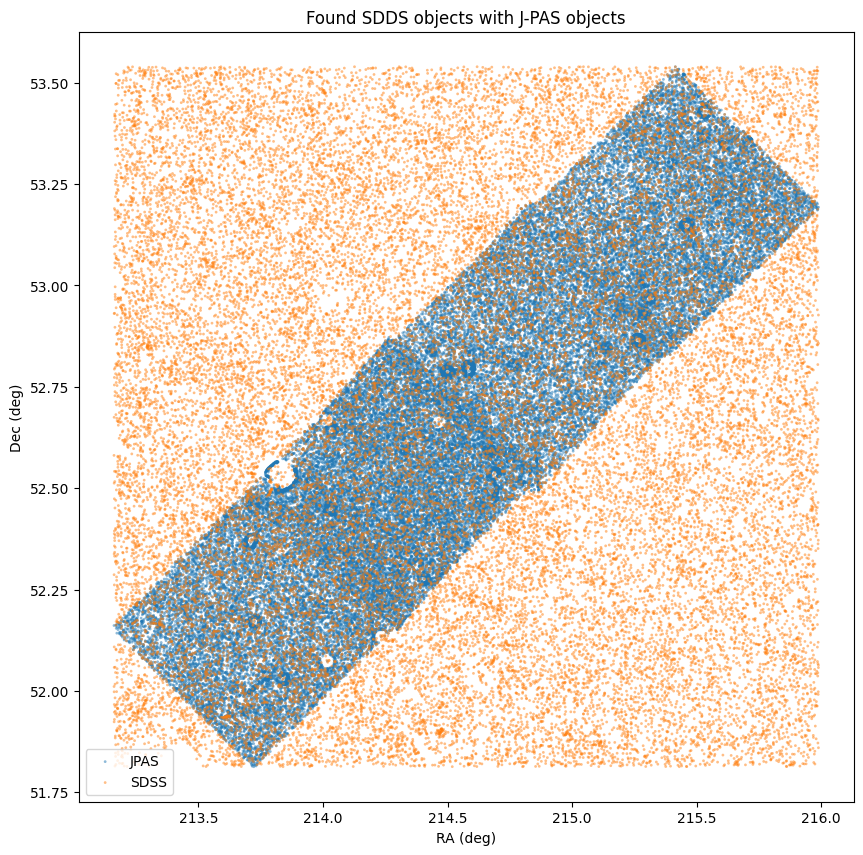
\includegraphics[width=0.75\textwidth]{../images/SDSS and J-PAS.png}
    \end{figure}
\end{frame}

\begin{frame}
\frametitle{Matching with SDSS Objects}
    We matched JPAS objects with SDSS objects by angular distance between objects (less than 1 arcsec). And then filtered the matched objects to include only unique matches.
    \begin{figure}
        \centering
        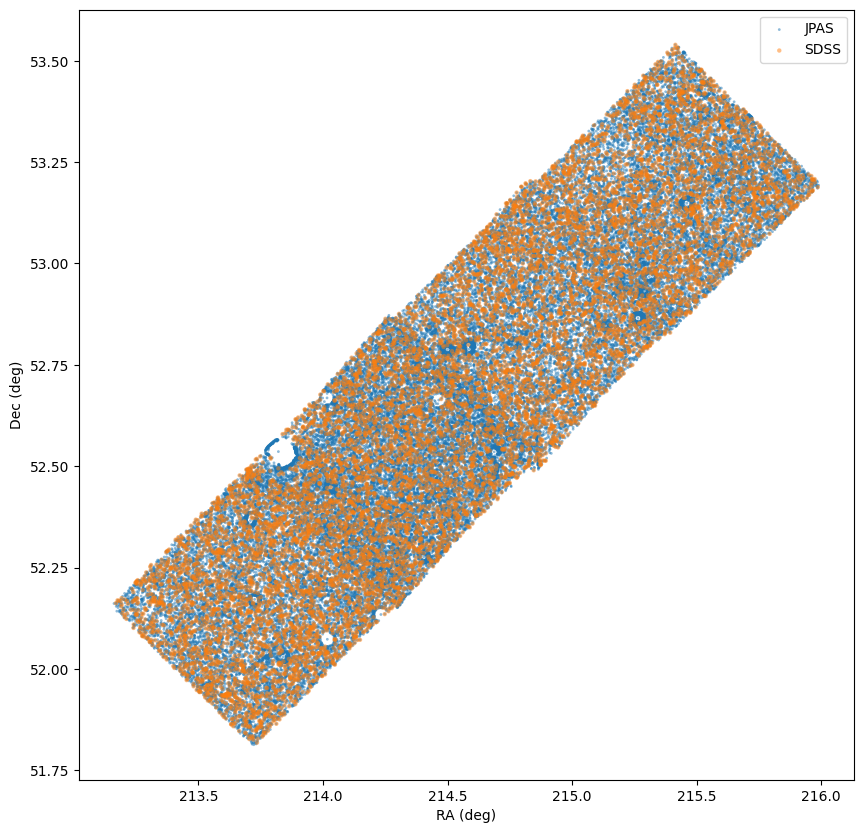
\includegraphics[width=0.6\textwidth]{../images/SDSS and J-PAS matched.png}
    \end{figure}
    In this way we got 11229 matched objects.
\end{frame}

\begin{frame}
\frametitle{}
    \begin{figure}
        \centering
        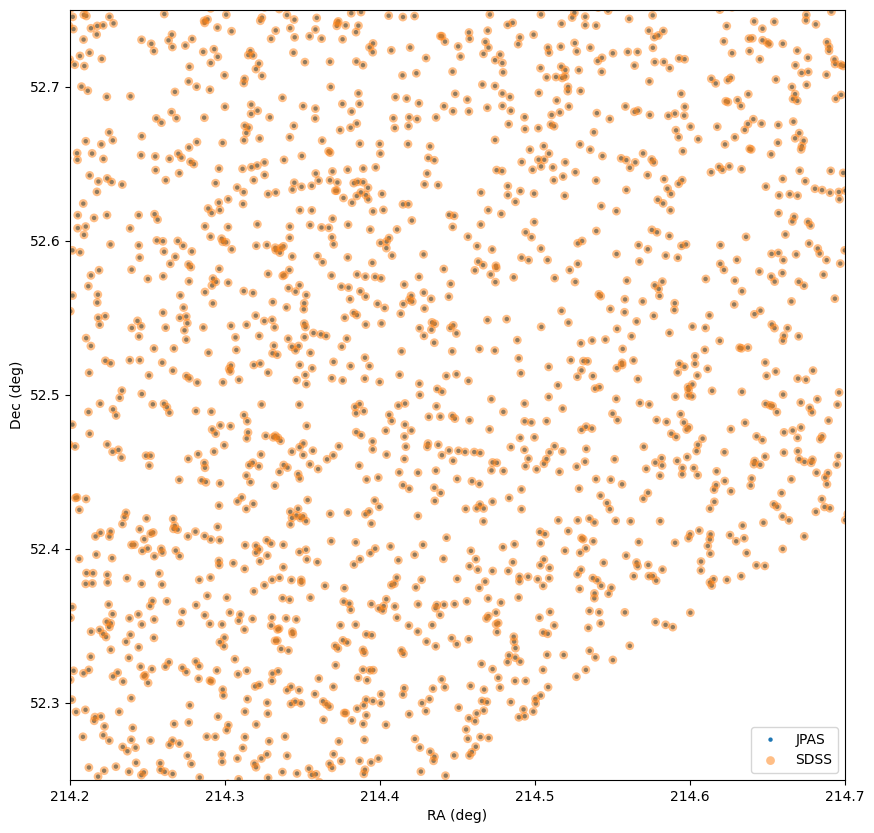
\includegraphics[width=0.7\textwidth]{../images/SDSS and J-PAS matched zoomed.png}
        \caption{Matched SDSS and J-PAS objects}
    \end{figure}
\end{frame}

\begin{frame}
\frametitle{Comparing Spectra}
    To compare spectra we first selected objects with spectra in the SDSS database and although filtered them by defined class of object.
    So in the end we get matched objects with spectra and defined class (1007 objects).
    \begin{center}
    \animategraphics[autoplay,loop,width=8cm]{0.5}{../images/spectra/jpas_sdss_}{0}{98}
    \end{center}
\end{frame}


\begin{frame}
    \frametitle{Resampling Spectra}
        We resampled JPAS and SDSS spectra to the same wavelength grid (50 Angstrom), so we can compare them properly.
        First, we interpolate the spectra to have evebly spaced wavelength grid for each spectra.
        Then we resample the spectra using scipy.signal.resample function.
        \begin{figure}
            \centering
            \only<1>
            {   
                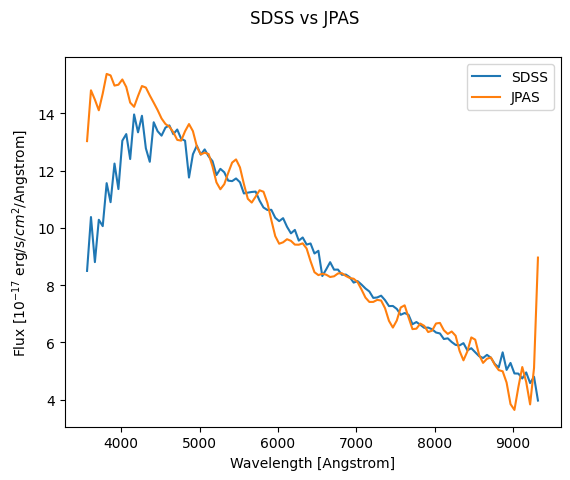
\includegraphics[width=0.6\textwidth]{../images/SDSS and JPAS.png}
            }
            \only<2>
            {   
                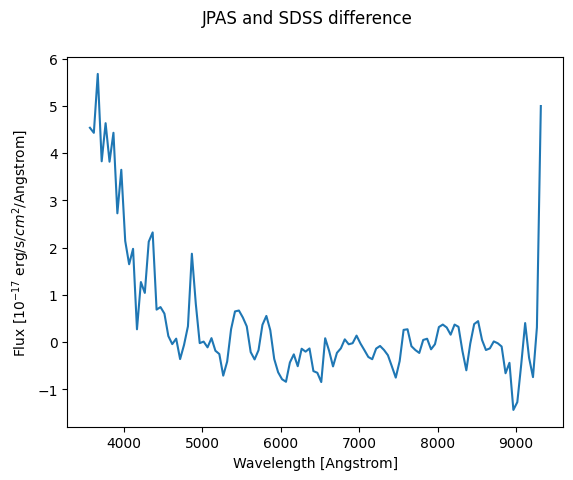
\includegraphics[width=0.6\textwidth]{../images/SDSS and J-PAS difference.png}
            }
        \end{figure}
\end{frame}

\begin{frame}
\frametitle{Future Work}
\begin{itemize}
    \item Map the spectral features of JPAS and SDSS objects to known classes of objects.
    \item Develop a classification model using machine learning to predict the class of JPAS objects based on their spectra.
    \item Test the classification model on new JPAS objects from new release.
\end{itemize}
\end{frame}

\begin{frame}
\begin{center}
    \Huge Thank you for your attention!
\end{center}
\end{frame}

\end{document}